\Aufgabe[e]{Integration}{
\begin{abc}
\item Berechnen Sie folgende Integrale
\begin{align*}
I_1=& \int x^2 \ln(x)\mathrm{d} x,\\
I_2=& \int \frac{x}{(x^2+1)^2} \mathrm{d} x,\\
I_3=& \int \frac{3x+2}{x^2+6x+9}\mathrm{d} x.
\end{align*}
\vspace*{-0.25cm}

\item Berechnen Sie das Integral
$$
I = \int_G y\ \mathrm{d} x \mathrm{d} y
$$
wobei $G\subset \mathbb R^2$ der Bereich ist, der zwischen den beiden Graphen der folgenden Funktionen liegt
$$
y = x^2 \quad \text{und} \quad y=2x.
$$
\end{abc}
}

\Loesung{
\begin{abc}
\item 
Das erste Integral ergibt sich durch einmalige partielle Integration: 
\begin{align*}
I_1=&  \int x^2 \ln{x}\mathrm{d} x\\
=& \frac{1}{3}x^3 \ln(x) - \frac{1}{3} \int x^3 \frac{1}{x} \mathrm{d} x\\
=& \frac{1}{3} x^3\ln{x} - \frac{1}{3} \int x^2 \mathrm{d} x\\
=& \frac{1}{3} x^3\ln{x} - \frac{1}{9} x^3 + c.
\end{align*}

F\"ur das zweite Integral ergibt die Substitution $u=x^2+1$, $\mathrm{d} u = 2x\mathrm{d} x$
\begin{align*}
	I_2=& \int \frac{1}{2} \frac{1}{u^2}\mathrm{d} x\\
	=& \frac{1}{2} (-1) \frac{1}{u} +c\\
	=& -\frac{1}{2} \frac{1}{u} + c \\
	=& -\frac{1}{2} \frac{1}{x^2+1} +c.
\end{align*}

Das dritte Integral ergibt sich durch die Partialbruchzerlegung: 
\begin{align*}
I_3=\int \frac{3x+2}{(x+3)^2}\mathrm{d} x
= \int\frac{3x+2}{(x+3)(x+3)}\mathrm{d} x\\
\end{align*}
\begin{align*}
\frac{3x+2}{(x+3)(x+3)} =& \frac{A}{x+3} + \frac{B}{(x+3)^2}\quad || \cdot (x+3)(x+3) \\
	\Longleftrightarrow 3x+2 =& A(x+3) + B \\
	 -7 =& B  \quad \Longrightarrow B = -7 \\
	 2=& 3A-7 \quad \Longrightarrow A = 3
\end{align*}
\begin{align*}
I_3=&\int\left(\frac{3}{(x+3)} - \frac{7}{(x+3)^2}\right)\mathrm{d} x\\
	 = &  3\ln{(|x+3|)} + \frac{7}{x+3} + c
 \end{align*} 
 
\item 
Die Fläche zwischen den beiden Graphen kann als Normalenbereich bezüglich x formuliert werden
$$
G := \{(x,y)\in \mathbb R^2: 0 \le x \leq 2\ \land\ x^2 \leq y \leq 2x \}
$$


\begin{align*}
I &= \int_G y\ \mathrm{d} x \mathrm{d} y,\\
&=\int_{x=0}^2 \int_{y=x^2}^{2x} y\ \mathrm{d} y \mathrm{d} x,\\
&=\int_0^2 \frac{1}{2}[y^2]_{x^2}^{2x}  \mathrm{d} y,\\
&= \frac{1}{2} \int_0^2 4x^2-x^4 \mathrm{d} y,\\
&= \frac{1}{2} \left[ \frac{4}{3} x^3 - \frac{1}{5}x^5 \right]_0^2 \\
&= \frac{1}{2} \left[ \frac{4}{3} 8 - \frac{1}{5} 32 \right] \\
&= \frac{1}{2} \frac{64}{15} \\
&= \frac{32}{15}
\end{align*}
\end{abc}

\begin{center}
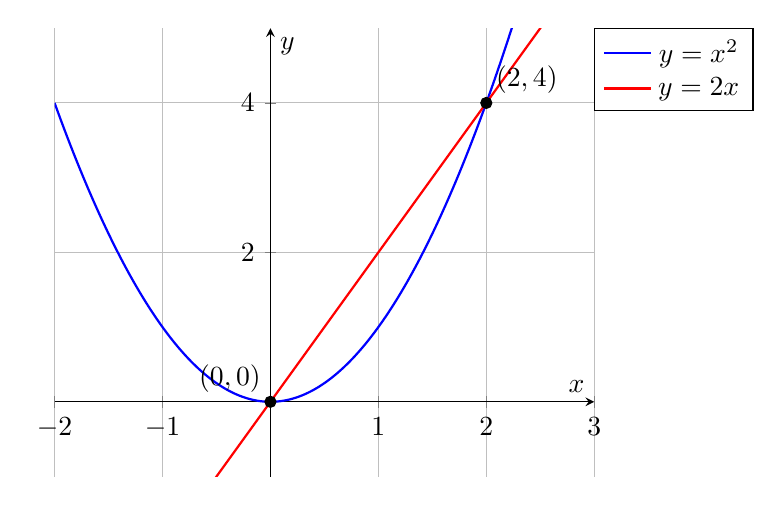
\begin{tikzpicture}
  \begin{axis}[
    axis lines = center,
    xlabel = $x$,
    ylabel = $y$,
    grid = both,
    legend style={at={(1,1)}, anchor=north west},
    xmin=-2, xmax=3,
    ymin=-1, ymax=5,
    samples=200
  ]
    % Funktionen
    \addplot[domain=-2:3, thick, blue]{x^2};
    \addlegendentry{$y = x^2$}

    \addplot[domain=-2:3, thick, red]{2*x};
    \addlegendentry{$y = 2x$}

    % Schnittpunkte
    \addplot[only marks, mark=*, mark size=2pt] coordinates {(0,0) (2,4)};
    \node[anchor=south east] at (axis cs:0,0) {$(0,0)$};
    \node[anchor=south west] at (axis cs:2,4) {$(2,4)$};

  \end{axis}
\end{tikzpicture}
\end{center}
}